\documentclass[12pt]{article}
%\documentclass{article}

\usepackage{times}
\usepackage[final]{graphicx}
\usepackage{hyperref}

\setlength{\topmargin}{-0.5in}
\setlength{\oddsidemargin}{0in}
\setlength{\evensidemargin}{0in}
\setlength{\textwidth}{6.5in}
\setlength{\textheight}{9.0in}

\begin{document}

\centerline{\bf \Large CS295/CS395/CSYS395: \href{CS295_395_Syllabus.pdf}{\underline{Evolutionary Robotics}}}

\vspace{0.5cm}

\centerline{\bf \large Programming Assignment 7 of 10}

\vspace{0.5cm}

\centerline{\large Assigned: Friday, October 14, 2011}

\vspace{0.5cm}

\centerline{\large Due: Friday, October 21, 2011 by midnight}

\vspace{0.5cm}

\noindent \textbf{Description:} In this week's assignment you will be adding motors to the robots to allow it to move. Each of the eight joints you created in last week's assignment will now be given a motor that sends forces to the joint in an attempt to make it reach a desired angle.

\begin{enumerate}

\item Back up Assignment\_6 on a flash drive or another computer so that you can always return to your completed fifth assignment.

\item Copy directory Assignment\_6, which contains your submitted document and the entire ODE folder. Rename the new directory Assignment\_7.

\item In the simLoop, add a line that commands joint 0 to reach an angle of -45$^o$. Ensure that this function is only called when the simulation is unpaused: \\
\texttt{if ( !pause ) \{} \\
\texttt{    ActuateJoint(0,-45);} \\
\texttt{    dSpaceCollide (space,0,\&nearCallback);} \\
\texttt{    dWorldStep (world,0.01);} \\
\texttt{    dJointGroupEmpty(contactgroup);} \\
\texttt{\}} \\
Note that the step size has been reduced to $0.01$ from the original setting of $0.05$. This will slow down your simulation but increase its accuracy. Once your robot starts moving, if the simulation is not accurate enough you may find your robot bouncing all over the place. If this is the case, come back to this line and try reducing the step size further.

\item Now define the function above simLoop: \\
\texttt{void ActuateJoint(int jointIndex, double desiredAngle) \{} \\
\texttt{...} \\
\texttt{\}}

\item The first line in this function should call the ODE function \\ \texttt{dJointSetHingeParam(...,dParamFMax,...)}. This function sets the maximum force that a motor can supply to the specified joint. Set this maximum force to 100 for now. You can reduce it later when your robots starts moving and the motions are too forceful.

\item The next lines should calculate the difference between the joint's current angle and the desired angle. You can get a joint's current angle using \texttt{dJointGetHingeAngle(...)}. Note that this function returns the angle in radians.

\item The greater this difference, the more force should be applied to reduce this difference; if the difference is zero, the joint should not be rotated at all. In order to accomplish this you will now include a line that instructs ODE to achieve a rotational velocity at the joint that is proportional to this difference: \\
    \texttt{dJointSetHingeParam(...,dParamVel,diff)}. \\
    Given this velocity, ODE will compute how much rotational force, or torque, to apply to the joint to achieve this velocity.

\begin{figure}[!t]
\centerline{
a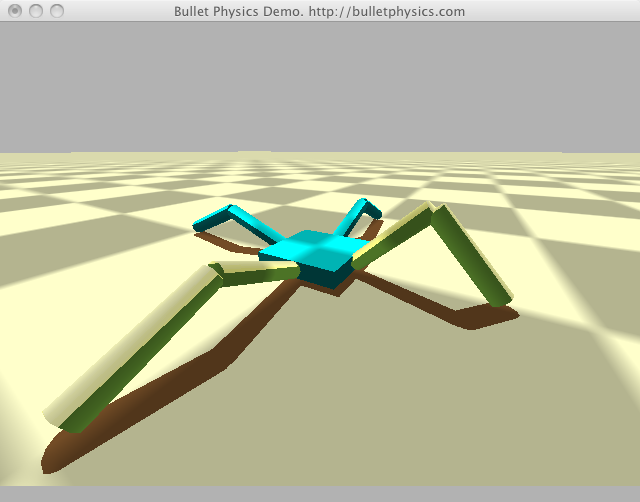
\includegraphics[width=0.25\textwidth]{Fig1a}
b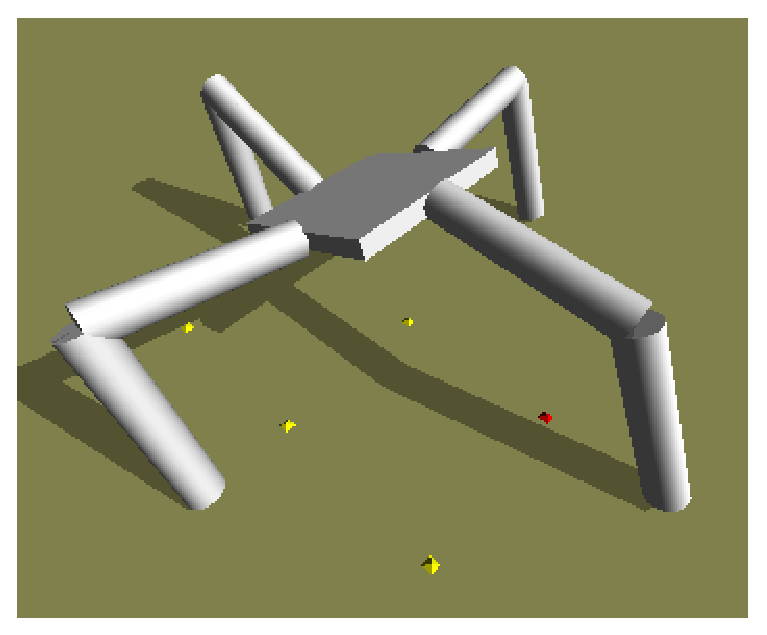
\includegraphics[width=0.25\textwidth]{Fig1b}
c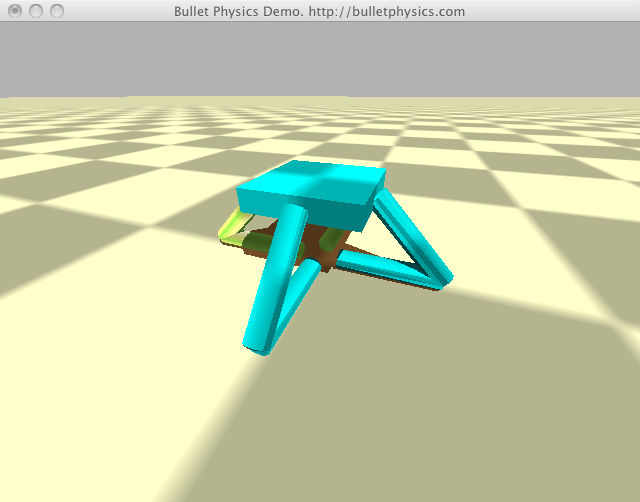
\includegraphics[width=0.25\textwidth]{Fig1c}}
\centerline{
d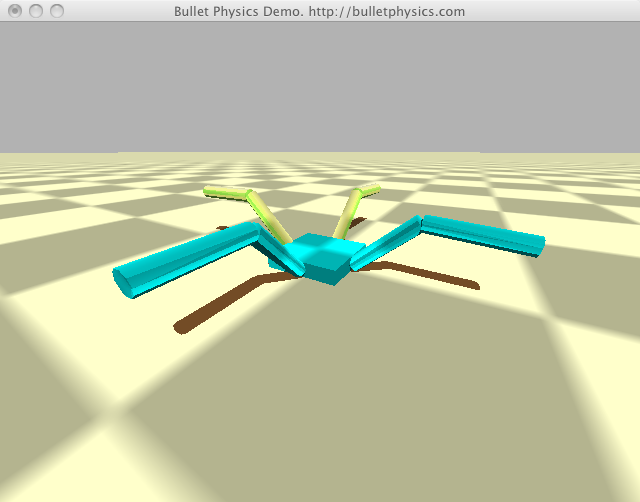
\includegraphics[width=0.25\textwidth]{Fig1d}
e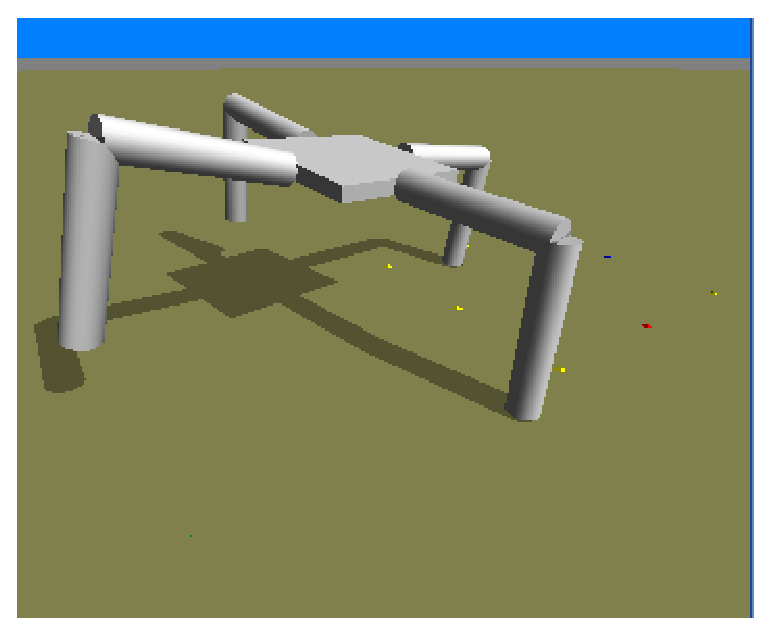
\includegraphics[width=0.25\textwidth]{Fig1e}}
\caption{Incremental addition of motors to the quadrupedal robot.}
\label{Fig1}
\end{figure}

\item Compile your code and run it. You should obtain an image as in Fig. \ref{Fig1}a: the first joint, which is the joint connecting the right upper leg to the main body, gradually rotates upward to 45$^o$. The other joints are still all passive, so that flop flat as before. Note that the right `knee' however bends more: as the right upper leg is raised, the right lower leg passively swings inward. \\ \\
    If you do not get this image, try increasing the maximum force that the motor can apply (step 5). You can also slow down \\
    (e.g. \texttt{dJointSetHingeParam(...,dParamVel,0.1*diff)}) \\
    or speed up \\
    (e.g. \texttt{dJointSetHingeParam(...,dParamVel,10.0*diff)}) \\
    the rate at which the motor rotates the joint to the desired angle. Once you get the robot to correctly raise its right upper leg, copy and paste your resulting image into your document. \\ \\
    Finally, you may find that the upper leg rotates downward instead of upward when you supply $-45^o$. You can get it rotate the leg upward by changing the direction of the joint axis by 180$^o$. For example if the joint's axis is $(0,0,1)$ and the leg rotates downward, change the axis to $(0,0,-1)$.

\item Once you've got this working, send $+45^o$ to the joint rather than $-45^o$: \\
    \texttt{ActuateJoint(0,+45)}. This produce the image seen in Fig. \ref{Fig1}b. Copy and paste this image into your document. From now on we will assume that negative angles extend a joint (i.e. push it `outward') and positive angles flex the joint (i.e. pull it `inward').

\item Now, instead of actuating just one joint, you will actuate all of them at each time step. Send $+45^o$ to all of the eight joints from within \texttt{simLoop} to flex all the joints inward. This should produce the image as in Fig. \ref{Fig1}c. If some of the joints extend outward, invert their joint axes as explained in step 8.

\item Change your code within \texttt{simLoop} again so that all of the joints extend outward, producing the image shown in Fig. \ref{Fig1}d. Copy and paste this into your document.

\item Finally, change the code in \texttt{simLoop} again so that, for each pass through simLoop, each motor is sent a different random angle drawn from the interval $[-45^o,45^o]$. You can create a random number between zero and one by calling \\
    \texttt{rand()/RAND\_MAX} \\
    you can scale this to a floating-point value in $[-45^o,45^o]$ using \\
    \texttt{(rand()/RAND\_MAX)*90-45} \\ \\
    When you run this you may find that your robots hops around because the legs are `jittering': they shake at a high frequency, but do not rotate far from their starting angle. If this occurs it is because the joint's speed (see step 8) is too slow: the joint does not have to time to rotate to the desired angle before the angle is changed at the next time step. If you have this problem, trying increasing the joints' speed. \\ \\
    Once the robots legs are moving sufficiently (and the motors' forces are high enough to allow the joints to move but not too high to cause the robot to flip over) the robot should start to move in random directions, as shown in Fig. \ref{Fig1}e. Note that this robot was, at the time this image was taken, statically unstable: only its two right feet were in contact with the ground. \\ \\
    Once the robot has moved sufficiently far from its start point (indicated by the nine colored dots embedded in the floor), copy and paste a snapshot from this simulation into your document.

\end{enumerate}

\end{document} 
